% Created 2021-03-02 Tue 11:16
% Intended LaTeX compiler: pdflatex
\documentclass[11pt]{article}
\usepackage[utf8]{inputenc}
\usepackage[T1]{fontenc}
\usepackage{graphicx}
\usepackage{grffile}
\usepackage{longtable}
\usepackage{wrapfig}
\usepackage{rotating}
\usepackage[normalem]{ulem}
\usepackage{amsmath}
\usepackage{textcomp}
\usepackage{amssymb}
\usepackage{capt-of}
\usepackage{hyperref}
\author{John Doe}
\date{\today}
\title{}
\hypersetup{
 pdfauthor={John Doe},
 pdftitle={},
 pdfkeywords={},
 pdfsubject={},
 pdfcreator={Emacs 27.1 (Org mode 9.5)}, 
 pdflang={English}}
\begin{document}

\tableofcontents

\section{Implementation}
\label{sec:org548b4ab}
\subsection{MD5}
\label{sec:org8e6b816}

\subsubsection{naive}
\label{MD5naive}
As explained in section\ref{SME}, SME consists of busses and processes. We can define the MD5 algorithm naively by following figure\ref{fig:Merkle} and using two busses and one simple process. Overall there are two approaches,
Firstly, we could let the arrows in the diagram denote the busses, such that we would have a bus denoting the message-block and one denoting the digest. However, this approach requires an extra bus, thus the alternative. Since we use a c\# implementation of SME, we can store the Digest locally inside the simpleProcess. Thus we will only require a bus with the message, corresponding to the downward-facing arrows and one for the Hash (the rightmost arrow).
we can define the Message bus as such:
\begin{verbatim}
    public interface IMessage : IBus {
        [InitialValue(false)] bool Valid { get; set; }

        [FixedArrayLength(MAX_BUFFER_SIZE)]
        IFixedArray<byte> Message { get; set; }

        int BufferSize { get; set; }
        int MessageSize { get; set; }

        [InitialValue(true)] bool Last { get; set; }
        [InitialValue(true)] bool Head { get; set; }
        [InitialValue(false)] bool Set { get; set; }
    }
\end{verbatim}
One can see there are multiple things to keep track of. First and foremost, all SME busses should have a flag for whether or not a bus has data inside of it. Secondly, A byte-array is used to store the message block itself. \texttt{BufferSize} will be updated for every iteration or tick, and denotes how many values in the buffer are set, essentially flag for when the message should be padded. MessageSize will be set in the initial tick and denote the length of the entire message used for the Merkle-Damgård strengthening.
The last 3 flags are used to handle some ``edge-cases''.
Head Denotes that the initialization vector should be reconstructed.
Last is used to denote when a block is the last in the message. The block cannot be filled with more than 447 bits.
Set is used in the cases where the initial 1 should be set but where the block is not the last in the message, for instance when the length of the message is 448.

The Digest on the other hand is simple. It only consists of a Valid flag and the Hash as an array of 4 32-bit words.

Except for the handling of the padding in relation to SME, the simple process works as explained in section\ref{MD5alg}

\subsubsection{First optimization approach}
\label{sec:org412c172}
To make the algorithm more efficient, the length of the circuit produced in the VHDL code should be reduced. Meaning we want the simple process to do less. For the initial approach, we can notice that the compression function in MD5 works in rounds. We can thus structure the program as such using a simple diagram. in figure\ref{fig:MD5opt1} one can see we can split the hash function as a whole up into 5 simple processes and build a pipeline from this. One process for message formatting, and one for each of the 4 rounds. along with an Imessage bus and a Digest bus as described in section\ref{MD5naive}. This construction will create a pipeline where each process can run concurrently and potentially execute faster than the naive approach.
\begin{figure}[htbp]
\centering
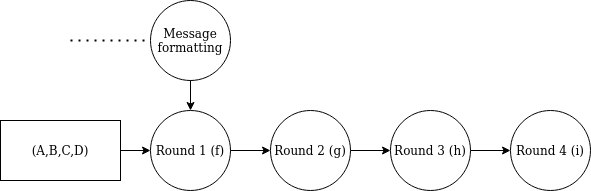
\includegraphics[width=.9\linewidth]{./MD5.png}
\caption{\label{fig:MD5opt1}MD5 pipeline}
\end{figure}

\subsubsection{Further optimizations}
\label{sec:org0f9db66}
This is just a question:
In Programming massively parallel hardware, I had a project where we were to implement a single pass parallel prefix Scan. And I know it is a bit different but, the idea is that each partition on the GPU will compute its own internal prefix scan and then wait for the previous one to finish and then add the prefix to every element in its internal scan. I was wondering if it could be worth trying a similar approach since a Merkel-Damgård construction is quite sequential in nature. So I thought if one could calculate everything that does not use the output from the previous tick, it might go faster, but I'm unsure whether such a thing could work on an FPGA since I still don't know too much about it.?
\end{document}
